\section{Le langage GRAFCET}

Le langage GRAFCET, aussi appelé SFC (Sequentiel Function Chart) est, comme son nom l'indique, dédié à la description et à la programmation de \textbf{problèmes séquentiels}. Il décrit donc une suite d'étapes séparées par des transitions.

Un GRAFCET est très proche conceptuellement d'une machine à état. Il est représenté tel que sur la Figure~\ref{fig:simpleGrafcet}

\begin{figure}[ht]
  \centering
  \begin{tikzpicture}
\EtapeInit[0,0]{100}
\Transition[VX100]{100}
\Etape[VT100]{110}
\Transition{110}
\Etape[VT110]{120}
\Transition[VX120]{120}
\LienRetour{T120}{X100}
\Recept{T100}{$dcy \cdot a_0$}
\ActionX{X110}{Sortir Noyau}
\Recept{T110}{condition}\ActionX{X120}{Rentrer Noyau}
\Recept{T120}{$a_0$}
\end{tikzpicture}

  \caption{GRAFCET simple composé de trois étapes}
  \label{fig:simpleGrafcet}
\end{figure}

\subsection{Étapes et actions}

Une étape est représentée par un carré comportant un numéro (Figure~\ref{fig:etape}). Elle est généralement associée à une  (Figure~\ref{fig:etapeAction}) ou plusieurs (Figure~\ref{fig:etapeDeuxActions}) actions.
Il est également possible d'ajouter une condition à une action (Figure~\ref{fig:etapeActionCond}).

\UPSTIaRetenir{\begin{itemize}
  \item Une action associée à une étape n'est effectuée que lorsque l'action associée est active.
  \item Une action conditionnelle est effectuée lorsque l'action est active et que la condition associée est vérifiée.
\end{itemize}}

Il également possible d'effectuer une action qu'au moment de l'activation d'une étape (Figure~\ref{fig:etapeActivation}). Cela est particulièrement utile pour incrémenter un compteur.
En effet, sans cela l'action \textit{compteur = compteur + 1} serait effectuée durant toute la durée de l'action associée. Cela incrémenterait le compteur à chaque cycle automate donc toutes les \SI{10}{ms} approximativement.

On peut représenter l'étape actuellement active dans un grafcet à l'aide d'une étoile comme illustré sur la Figure~\ref{fig:etapeActive}.

\begin{figure}[ht]
\centering
  \begin{subfigure}[b]{.49\textwidth}
    \centering
    \begin{tikzpicture}
      \Etape[0,0]{110}
    \end{tikzpicture}
    \caption{Représentation d'une étape en GRAFCET}
    \label{fig:etape}
  \end{subfigure}%
  %
  \begin{subfigure}[b]{.49\textwidth}
    \centering
  \begin{tikzpicture}
    \Etape[0,0]{110}
    \ActionX{X110}{Sortir Noyau}
  \end{tikzpicture}
  \caption{Une étape et l'action associée}
  \label{fig:etapeAction}
  \end{subfigure}%
  %

  \begin{subfigure}[b]{.48\textwidth}
    \centering
  \begin{tikzpicture}
    \Etape[0,0]{110}
    \ActionX{X110}{Sortir Noyau, Allumer voyant}
  \end{tikzpicture}
  \caption{Une étape et deux actions simultanées. Les deux actions sont actives tant que l'étape 110 est active.}
  \label{fig:etapeDeuxActions}
  \end{subfigure}\hfill
%
  \begin{subfigure}[b]{.48\textwidth}
    \centering
  \begin{tikzpicture}
    \Etape[0,0]{110}
    \ActionX{X110}{Sortir Noyau}
    \ActionCond{X110}{$\overline{\text{defaut}}$}
  \end{tikzpicture}
  \caption{Une étape avec action conditionnelle : L'action \textit{Sortir Noyau} ne sera exécutée que si \textit{defaut} est à 0.}
  \label{fig:etapeActionCond}
  \end{subfigure}%

  \begin{subfigure}[b]{.48\textwidth}
    \centering
  \begin{tikzpicture}
    \Etape[0,0]{130}
    \ActionX{X130}{compteur = compteur + 1;}
    \ActionActiv{X130}
  \end{tikzpicture}
  \caption{Une étape et une action sur activation. L'action n'est effectuée qu'au moment de l'activation de l'étape.}
  \label{fig:etapeActivation}
  \end{subfigure}%
  %
  \begin{subfigure}[b]{.48\textwidth}
    \centering
  \begin{tikzpicture}
    \Etape[0,0]{110}
    \ActionX{X110}{Sortir Noyau}
    %\ActionCond{X110}{$\overline{\text{defaut}}$}
    \LienActivation{X110}
  \end{tikzpicture}
  \caption{Etape courramment active}
  \label{fig:etapeActive}
  \end{subfigure}
  \caption{Etapes et action(s) associée(s)}%
  %
\end{figure}


\subsection{Transitions}

Une transition est \textbf{toujours} placée entre deux actions. Ce sont les transitions qui décrivent la façon de passer d'une action à une autre.
Une transition est associée à une \textbf{réceptivité}.

\UPSTIaRetenir{Une transition sera franchie si et seulement si l'étape précédente est active ET la réceptivité associée est vérifiée.}
